%!TEX root = ./../thesis.tex

\chapter{Framework}
\label{c:state_centric}
Most state-of-the-art frameworks for distributed machine learning like Petuum \cite{Xing2015} and Parameter Server \cite{Li2014} are based on the parameter server concept introduced in the previous section.
The framework essentially provides a low level API\footnote{Application programming interface} for publishing and retrieving values similar to a distributed key-value store, where the key $i$ is for example the index of a weight vector $w$ stored on the server and the value is the weight $w_i$.
Implementing an algorithm that relies on a parameter server requires incorporating publishing and retrieval of parameters deeply into the algorithm definition.
This contrasts the general work flow of developing and testing an algorithm locally on a single machine and then transition to a distributed environment such as a cluster.
Also the parameter server paradigm provides only a minor abstraction, leaving the developer with the task of distributing state, scheduling distributed computation, consistency management and managing cluster resources.
A developer should be able to focus on the main goal of distributed machine learning, namely an efficient parallel execution.
This section introduces the general architecture of the framework and its main parts based on the example of iterative-convergent algorithms, though its application is not limited to this particular family of algorithms.

As depicted in Figure \ref{fig:framework_architecture} the framework consists of three major parts, supporting the developer with the development and execution of distributed machine learning algorithms.
First, it provides a collection of primitives that can used to describe the algorithm with the help of a state centric programming model.
The SCPM\footnote{State-centric Programming Model} treats state as a first class citizen which can be distributed according to a given partitioning and altered by local and remote transformation in parallel.
Depending on how a state is distributed and the type of transformation applied to it, the consistency management ensures a correct execution of each algorithm steps among all participating machines.
For this purpose, additional primitives are offered by the framework to provide the consistency management with instructions on how to ensure a consistent distributed execution given a particular state and transformation.
\begin{figure}[ht]
\centering
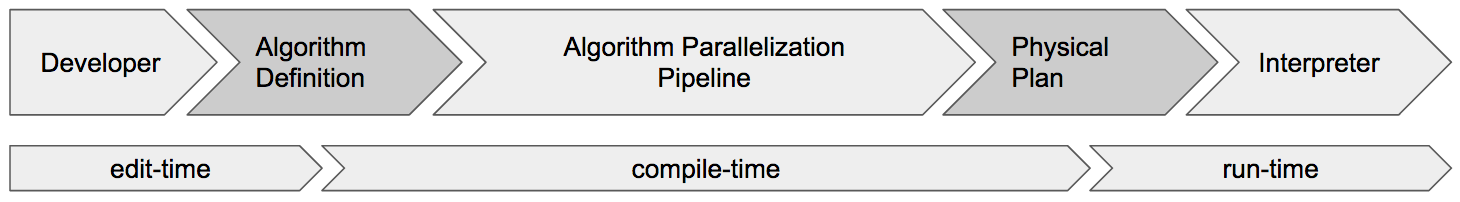
\includegraphics[width=0.9\textwidth]{img/framework_architecture.png}
\caption{Framework Architecture}
\label{fig:framework_architecture}
\end{figure}
Secondly, the framework provides an algorithm parallelization pipeline which takes the algorithm definition as an input an creates a physical plan by applying a series of transformation or enrichment steps to it.
The physical plan contains a detailed description on how to execute the algorithm in a distributed manner on a specific group of machines within the cluster.
As the third part of the framework, the interpreter is responsible for translating the physical plan into control instructions for the machines part of the compute cluster, as can be seen in Figure \ref{fig:framework_driver}.
\begin{figure}[ht]
\centering
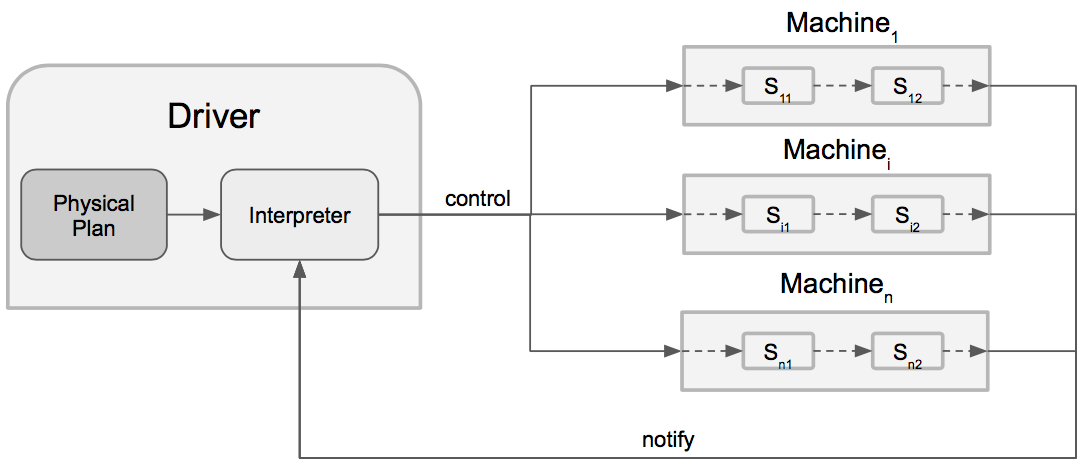
\includegraphics[width=0.8\textwidth]{img/framework_driver.png}
\caption{Algorithm Execution Architecture}
\label{fig:framework_driver}
\end{figure}
In this context, the driver is an arbitrary machine responsible for running the interpreter, which can be either a dedicated machine part of the cluster or the developers own machine.

\section{State Centric Programming Model}
In order to support the development process, a programming model is required that is expressive enough to conveniently model the complex dependencies when executing a machine learning algorithm in a distributed manner.
For this purpose the framework provides a so called state centric programming model, which is derived by the help of the example algorithm definition in \ref{alg:general_ica}.
The definition represents an iterative-convergent algorithm as it would be implemented by a developer.
Due to the fact that the general algorithm definition is very similar among members of the ICA\footnote{iterative-convergent-algorithm} family, only $f_p$ and $\Delta(\ldots)$ must be replaced by the corresponding preprocessing transformation respectively the optimization technique used for iteratively approximating the optimal solution according to Section \ref{ss:optimization}.
\begin{algorithm}
\caption{Generic iterative-convergent algorithm definition}\label{alg:general_ica}
\begin{algorithmic}[1]{}
\ALGSTATE Data tensor $D \in \mathbb{R}^{n \times d}$, weight tensor $w \in \mathbb{R}^{m \times d}$
\INPUT algorithm specific hyper-parameters $\theta$, if any
\INIT $t \gets 0$, $w^{(0)} \gets 0$
\State $D \gets f_{p}(D)$ \Comment{(A)}
\Repeat \Comment{(B)}
\State $t \gets t + 1$
\State $w^{(t)} \gets w^{(t-1)} + \Delta(w^{(t-1)}, \theta, D)$ \Comment{(C)}
\Until{termination criteria satisfied} \Comment{(D)}
\end{algorithmic}
\end{algorithm}
Figure \ref{fig:ica_control_flow} shows the control flow of (\ref{alg:general_ica}), describing the training process of an ICA such as linear regression, support-vector machine or logistic regression.
\begin{figure}[ht]
\centering
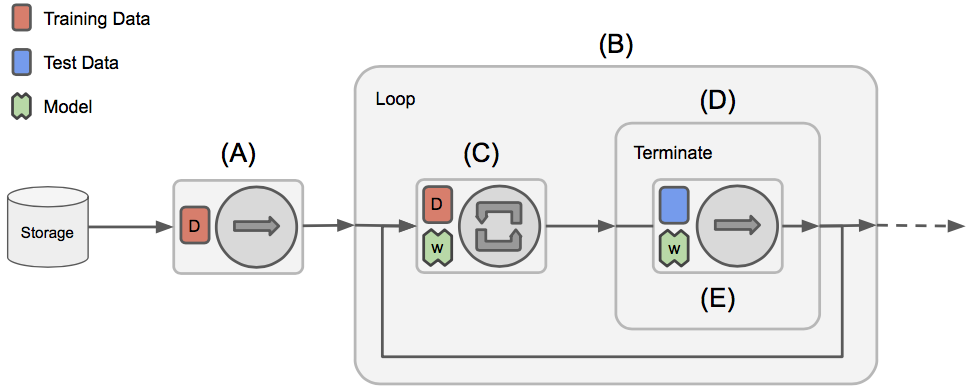
\includegraphics[width=0.9\textwidth]{img/ica_control_flow.png}
\caption{Logical plan for iterative-convergent algorithms}
\label{fig:ica_control_flow}
\end{figure}
The process starts with loading the input data $D$ from the storage followed by one ore more preprocessing steps (e.g. normalization or standardization as well as splitting the data into training and test set \textbf{(A)}).
A square represents a step of the algorithm, which contains an arbitrary number of input states (e.g. data, model) and some kind of transformation applied to them.
The transformation process is depicted as a circle and can either be applied once (arrow) or multiple times (cyclic arrows) to the state(s) during this particular step.
After applying the preprocessing the actual training process is triggered, which is contained in a loop \textbf{(B)}.
A loop symbolizes that the containing steps are executed repeatedly until some termination criterion \textbf{(D)} is satisfied, which is computed in \textbf{(E)}.
For most machine learning algorithms the termination criterion can either be a fixed number of iterations, the change in objective $Q$ between iterations or the generalization performance.
\textbf{(C)} is the actual training step which iteratively refines the model by updates computed from the input data according to \ref{eqn:delta_upd}.
It can already be seen from the example that the framework must be capable of executing a complex sequence of arbitrary control flow operators and transformation steps.
An algorithm expressed in this form could be executed as is on a single machine without modification because its sequential, non-parallel execution ensures the consistency of all involved states throughout the algorithm execution.
Consistency in this context means that, because of its sequential execution, no conflicts can occur when altering a particular state as described in Section \ref{ss:consistency}.
Distributing said algorithm therefore requires additional instructions on how to ensure that conflicts can be resolved properly.
These instructions are then combined with the logical representation of the algorithm and additional information regarding the distribution of state and the cluster environment to obtain a physical representation.
This is the responsibility of the algorithm parallelization pipeline, described in Section \ref{s:algo_parallel_pipeline}, which takes the algorithm definition as input and returns a physical plan.
The next sections introduce the key elements of the programming model discussed by the help of the example algorithm.

\subsection{State}
Assuming the algorithm described in (\ref{alg:general_ica}) should be parallelized with a dop\footnote{degree of parallelism} of two.
In order to achieve this degree of parallelism, it is necessary to replicate each transformation step of the sequential algorithm on multiple machines, as shown in Figure \ref{fig:ica_control_flow_dist}.
\begin{figure}[ht]
\centering
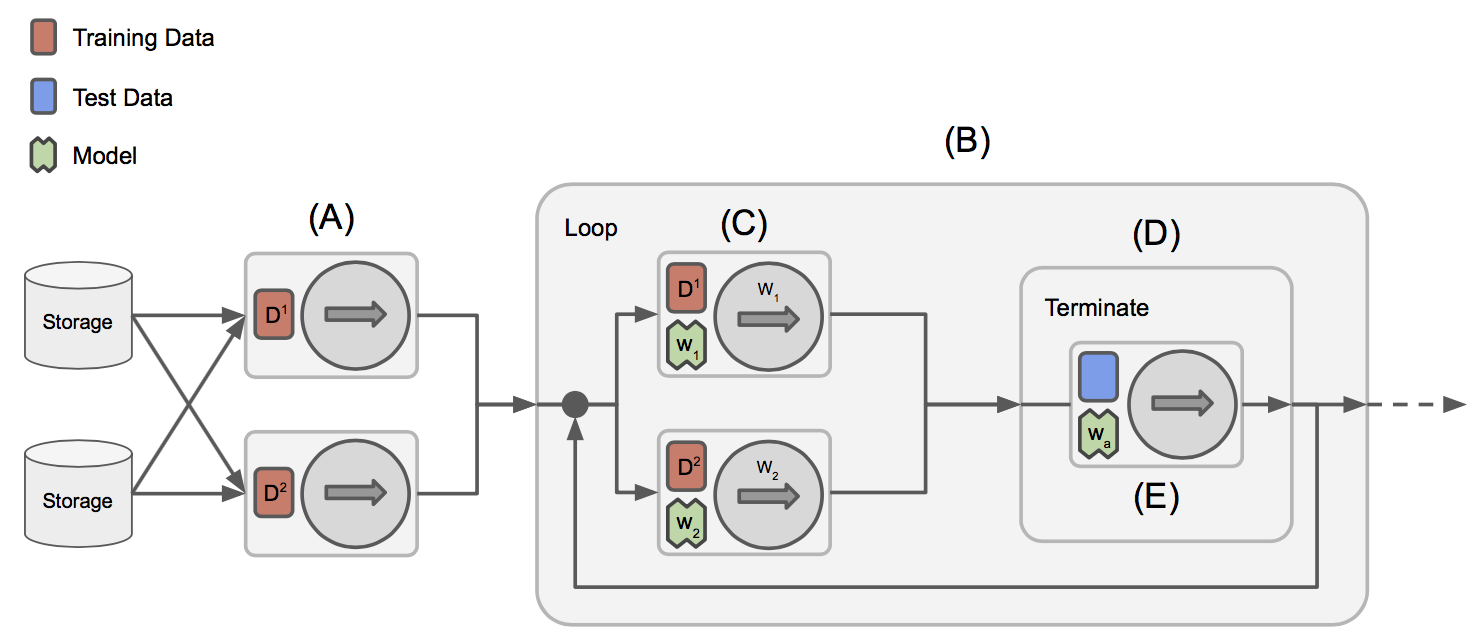
\includegraphics[width=0.9\textwidth]{img/ica_control_flow_dist.png}
\caption{Distributed Machine Learning Pipeline for Iterative-convergent Algorithms}
\label{fig:ica_control_flow_dist}
\end{figure}
It is worth noting that the transformation logic stays the same independently of the degree-of-parallelism, including a dop of one, which is essentially a single machine.
Therefore the framework instead of parallelizing the transformation focuses on how to parallelize the state and keeping it consistent.
Hence the programming model introduces the concept of state, which is essentially a container for an arbitrary, distributable data structure.
A state $\gamma$ must be partitionable, meaning it can be distributed according to a partitioning $\{P_{\gamma}\}_{k=1}^K$, where $K$ is the degree of parallelism.
In the area of machine learning, state is commonly represented by tensors of arbitrary type, such as floating point numbers, integers or strings.
Therefore any further discussion assumes that a state is represented by a tensor of order two (matrix).
For example the algorithm in (\ref{alg:general_ica}) requires two states, namely the input data $D$ and the model $w$.
In order to parallelize the algorithm, the parallelization pipeline requires a partitioning $\{P\}_{k=1}^K$ for both states, which in machine learning can be divided into the following cases, shown in Table \ref{tab:ica_partitioning}.
\begin{table}[h]
\begin{center}
\begin{tabular}{ | c | c | c |}
\hline
$\gamma_w \setminus \gamma_D$ & partitioned & replicated \\ \hline
partitioned & $\gamma_w^S \wedge \gamma_D^T$ &  $\gamma_w^S \wedge \gamma_{D_T}$\\ \hline
replicated & $\gamma_{w_S} \wedge \gamma_D^T$ & $\times$\\
\hline
\end{tabular}
\label{tab:ica_partitioning}
\caption{Distributed Machine Learning Pipeline for Iterative-convergent Algorithms}
\end{center}
\end{table}
Where $S \subset \{1, \ldots, M\}$ and $T \subset \{1, \ldots, M\}$, with $M$ being the number of available machines in the cluster and $\mid S \mid = \mid T \mid = K$.
In this context, a subscript set of indices means the state is replicated among the set of machines, whereas a superscript set of indices indicates the state is partitioned among the set of machines.
As described in Section \ref{ss:state_partitioning}, $w_S \wedge D^T$ equals data-parallelism, $w^S \wedge D_T$ equals model-parallelism and $w^S \wedge D^T$ is a hybrid approach that is often used in a parameter server setup where model and input data are both distributed among a set of machines.
The example in Figure \ref{fig:ica_control_flow_dist} therefore depicts a data-parallel approach because the input data $D$ is partitioned into $D^{\{1,2\}}$, whereas the model $w$ is replicated across machines $w_{\{1,2\}}$.
In general the distribution of state in machine learning depends on the size of the problem and the algorithm employed to obtain an optimal solution for the given objective.
E.g. in cases where the model $w$ does not fit into the memory of a single machine it is partitioned among a sufficient number of machines.
The same holds for the size of the input data $D$.
A special case is the partitioning $\{P_D\}_{k=1}^K$ of the input data, which is in general a matrix with rows consisting of examples.
For iterative-convergent algorithms, depending on the optimization technique used to iteratively optimize the objective $Q$ of interest, two partitioning schemes are commonly used.
If the optimization technique requires access to a complete example in order to update the model, such as it is the case with stochastic gradient descent, the input data is partitioned row-wise.
On the other hand, if a coordinate-wise optimization technique is used which only needs access to a single feature, the input data is distributed column-wise as shown in Figure \ref{fig:row_col_dist} for a dop of two.
\begin{figure}[ht]
\centering
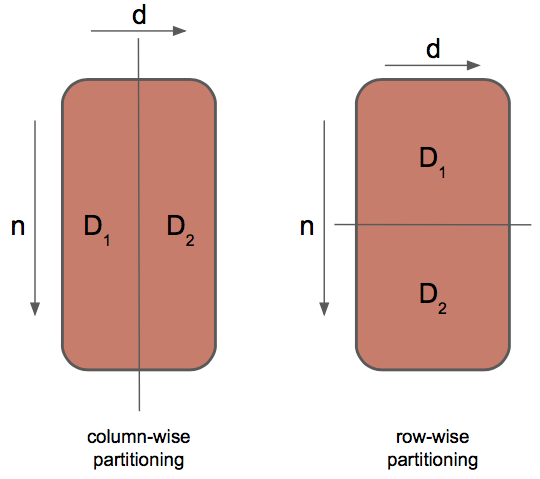
\includegraphics[width=0.5\textwidth]{img/row_col_dist.png}
\caption{Partitioning of input data in distributed machine learning}
\label{fig:row_col_dist}
\end{figure}

\subsection{Transformation}

\subsection{Consistency}

\begin{algorithm}
\caption{SCPM iterative-convergent algorithm definition}\label{alg:scpm_ica}
\begin{algorithmic}[1]{}
\ALGSTATE Data tensor $D \in \mathbb{R}^{n \times d}$, weight tensor $w \in \mathbb{R}^{m \times d}$
\PARTITIONING $\{P_D\}_{k=1}^K$, $\{P_w\}_{k=1}^K$
\CONSISTENCY 
\INPUT algorithm specific hyper-parameters $\theta$, if any
\INIT $t \gets 0$, $w^{(0)} \gets 0$
\State $D \gets f_{p}(D)$
\Repeat
\State $t \gets t + 1$
\State $w^{(t)} \gets w^{(t-1)} + \Delta(w^{(t-1)}, \theta, D)$
\Until{termination criteria satisfied}
\end{algorithmic}
\end{algorithm}


\section{Algorithm Parallelization Pipeline}
\label{s:algo_parallel_pipeline}
This intermediate representation (logical plan) can then be combined with information about the cluster resources and instructions for the consistency management to obtain a physical plan, which is then used by the framework to actually schedule the distributed execution of the algorithm in a cluster.
The sequence of steps necessary to go from an algorithm definition to a distributed or physical plan is depicted in Figure \ref{fig:parallel_pipeline}, where a light arrow resembles an intermediate representation and a dark arrow depicts a transformation step between those representations.
At each step, the corresponding representation is enriched by additional information about the algorithm or cluster infrastructure.
\begin{figure}[ht]
\centering
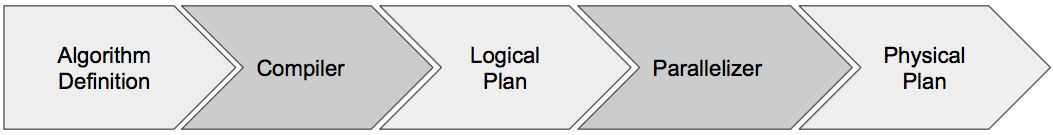
\includegraphics[width=0.9\textwidth]{img/algo_parallel_pipeline.png}
\caption{Algorithm parallelization pipeline}
\label{fig:parallel_pipeline}
\end{figure}
The following sections describe how the intermediate representations look like and what purpose they serve.

\subsection{Compiler}
In the first step, a logical plan is derived from the algorithm definition, the compiler identifies the building blocks of the given algorithm such as control flow, transformations and state present in the algorithm as well as the dependencies among them.
The information used to derive the logical plan is solely based on the algorithm definition and does not take infrastructure related properties into account because this representation should be architecture independent.




\textbf{NOTES:} add caption for state, change figure, make termination more generic, it's better to call this control flow
- describe the development flow: developer implements algorithm (specifies states, control flow, applied transformations -> functions), this needs to be identified and mapped into a logical plan by the compiler

\subsection{Parallelizer}
Therefore the actual concern in distributed machine learning is not how to distribute computation but how to distribute the state an keep it consistent in order to achieve optimal performance.
As this thesis focuses on machine learning, a state is in general represented by a tensor (e.g. vector or matrix).
The most efficient state distribution depends on properties of the state(s) such as size and sparsity of the input data and model, algorithm used for optimization and infrastructure properties such as available memory and computational resources.

\textbf{NOTES:} add caption for state, change figure, make termination more generic, it's better to call this control flow

NOTES:
- motivate the argumentation with an example machine learning pipeline (elastic-net linear regression) which includes preprocessing (e.g. standard-scaling), iterative model refinement which could be data/model parallel and depending on the size of the model it could either be replicated or partitioned among machines/workers, also a ML pipeline involves generalization error assessment via test/validation dataset, which should be included into the stopping criterion
this should show:
	- what kind of workflow is generaly executed in practice
	- what structure a ml pipeline has and that there are parts that can be run in parallel and in parallel with relaxed constistency/synchronization
	- show what kind of information can be infered from knowledge about the architecture (computational and memory resources, bandwidth, bandwidth quota) and the problem size (size of input data, size of model)
	- what part of distributing a machine learning algorithm can be handled by the system (distributing data, distributing model and computation, scheduling of work) and what needs to be specified by the developer (parallelism, control flow and required states (?), )

- describe the limitations of current state-of-the-art distributed machine learning systems
	- low level primitives
	- not flexible nor expressible api for developing real word machine learning pipelines
	- inference of certain properties depending on hardware architecture (GPU, CPU, FPGA) and algorithm properties
	- distributed control flow
	- focus on optimizing distributed machine learning performance by quick prototyping
	- only concerned with the important parts for going from an exact single machine to a distributed algorithm implementation by specifying data partitioning, topology and constistency management properties (synchronzation requirements/schemes, filter, update/merging strategies)
	- dealing with algorithm related hyperparameters
